% В этом файле следует писать текст работы, разбивая его на
% разделы (section), подразделы (subsection) и, если нужно,
% главы (chapter).

% Предварительно следует указать необходимую информацию
% в файле SETUP.tex

%% В этот файл не предполагается вносить изменения

% В этом файле следует указать информацию о себе
% и выполняемой работе.

\documentclass [fontsize=14pt, paper=a4, pagesize, DIV=calc]%
{scrartcl}
% ВНИМАНИЕ! Для использования глав поменять
% scrartcl на scrreprt

% Здесь ничего не менять
\usepackage [T2A] {fontenc}   % Кириллица в PDF файле
\usepackage [utf8] {inputenc} % Кодировка текста: utf-8
\usepackage [russian] {babel} % Переносы, лигатуры


\usepackage{fancyhdr}

\addto\captionsrussian{\renewcommand{\contentsname}{Contents}}

%%%%%%%%%%%%%%%%%%%%%%%%%%%%%%%%%%%%%%%%%%%%%%%%%%%%%%%%%%%%%%%%%%%%%%%%
% Создание макроса управления элементами, специфичными
% для вида работы (курс., бак., маг.)
% Здесь ничего не менять:
\usepackage{ifthen}
\newcounter{worktype}
\newcommand{\typeOfWork}[1]
{
	\setcounter{worktype}{#1}
}

% ВНИМАНИЕ!
% Укажите тип работы: 0 - курсовая, 1 - бак., 2 - маг.,
% 3 - бакалаврская с главами.
\typeOfWork{1}
% Считается, что курсовая и бак. бьются на разделы (section) и
% подразделы (subsection), а маг. — на главы (chapter), разделы и
%  подразделы. Если хочется,
% чтобы бак. была с главами (например, если она большая),
% надо выбрать опцию 3.

% Если при выборе 2 или 3 вы забудете поменять класс
% документа на scrreprt (см. выше, в самом начале),
% то получите ошибку:
% ./aux/appearance.tex:52: Package scrbase Error: unknown option ` chapterprefix=

%%%%%%%%%%%%%%%%%%%%%%%%%%%%%%%%%%%%%%%%%%%%%%%%%%%%%%%%%%%%%%%%%%%%%%%%
% Информация об авторе и работе для титульной страницы

\usepackage {titling}

% Имя автора в именительном падеже (для маг.)
\newcommand {\me}{%
И.\,И.~Иванов%
}

% Имя автора в родительном падеже (для курсовой и бак.)
\newcommand {\byme}{%
И.\,А.~Стребежева%
}

% Научный руководитель
\newcommand{\supervisor}%
{к.т.н, ст. преподаватель Е.\,В.~Алымова}

% идентифицируем пол (только для курсовой и бак.)
\newcommand{\bystudent}{
Студента %Студентки % Для курсовой: с большой буквы
}

% Год публикации
\date{2017}

% Название работы
\title{Разработка плагина поддержки языка Coq\\для редактора Atom}

% Кафедра
%

\newcommand {\direction} {%
Направление подготовки\\02.\ifthenelse{\value{worktype} = 2}{04}{03}.02 ---
Фундаментальная информатика\\и информационные технологии%
}

%%%%%%%%%%%%%%%%%%%%%%%%%%%%%%%%%%%%%%%%%%%%%%%%%%%%%%%%%%%%%%%%%%%%%%%%
% Другие настраиваемые элементы текста

% Листинги с исходным кодом программ: укажите язык программирования
\usepackage{listings}
\lstset{
    language=[ISO]C++,%  Язык указать здесь
    basicstyle=\small\ttfamily,
    breaklines=true,%
    showstringspaces=false%
    inputencoding=utf8x%
}
% полный список языков, поддерживаемых данным пакетом, есть,
% например, здесь (стр. 13):
% ftp://ftp.tex.ac.uk/tex-archive/macros/latex/contrib/listings/listings.pdf

% Нумерация списков: можно при необходимести
% изменять вид нумерации (например, добавлять правую скобку).
% По умолчанию буду списки вида:
% 1.
% 2.
% Изменять вид нумерации можно в начале нумерации:
% \begin{enumerate}[1)] (В квадратных скобках указан желаемый вид)
\usepackage[shortlabels]{enumitem}
                    \setlist[enumerate, 1]{1.}

% Гиперссылки: настройте внешний вид ссылок
\usepackage%
[pdftex,unicode,pdfborder={0 0 0},draft=false,%backref=page,
    hidelinks, % убрать, если хочется видеть ссылки: это
               % удобно в PDF файле, но не должно появиться на печати
    bookmarks=true,bookmarksnumbered=false,bookmarksopen=false]%
{hyperref}


\usepackage {amsmath}      % Больше математики
\usepackage {amssymb}
\usepackage {textcase}     % Преобразование к верхнему регистру
\usepackage {indentfirst}  % Красная строка первого абзаца в разделе

\usepackage {fancyvrb}     % Листинги: определяем своё окружение Verb
\DefineVerbatimEnvironment% с уменьшенным шрифтом
	{Verb}{Verbatim}
	{fontsize=\small}

% Вставка рисунков
\usepackage {graphicx}

% Общее оформление
% ----------------------------------------------------------------
% Настройка внешнего вида

%%% Шрифты

% если закомментировать всё — консервативная гарнитура Computer Modern
\usepackage{paratype} % профессиональные свободные шрифты
%\usepackage {droid}  % неплохие свободные шрифты от Google
%\usepackage{mathptmx}
%\usepackage {mmasym}
%\usepackage {psfonts}
%\usepackage{lmodern}
%var1: lh additions for bold concrete fonts
%\usepackage{lh-t2axccr}
%var2: the package below could be covered with fd-files
%\usepackage{lh-t2accr}
%\usepackage {pscyr}

% Геометрия текста

\usepackage{setspace}       % Межстрочный интервал
\onehalfspacing

\newlength\MyIndent
\setlength\MyIndent{1.25cm}
\setlength{\parindent}{\MyIndent} % Абзацный отступ
\frenchspacing            % Отключение лишних отступов после точек
\KOMAoptions{%
    DIV=calc,         % Пересчёт геометрии
    numbers=endperiod % точки после номеров разделов
}

                            % Консервативный вариант:
%\usepackage                % ручное задание геометрии
%[%                         % (не рекомендуется в проф. типографии)
%  margin = 2.5cm,
  %includefoot,
  %footskip = 1cm
%] %
%  {geometry}

%%% Заголовки


\ifthenelse{{\value{worktype} > 1}}{%
  \KOMAoptions{%
      headings=normal,   % размеры заголовков поменьше стандартных
      chapterprefix=true,% Печатать слово Глава
      appendixprefix=true% Печатать слово Приложение
  }
}{% Печатать слово Приложение даже если нет глав
  \newcommand*{\appendixmore}{%
    \renewcommand*{\sectionformat}{%
    \appendixname~\thesection\autodot\enskip}
    \renewcommand*{\sectionmarkformat}{%
      \appendixname~\thesection\autodot\enskip}
  }
}

% шрифт для оформления глав и названия содержания
\newcommand{\SuperFont}{\Large\sffamily\bfseries}

% Заголовок главы
\ifthenelse{\value{worktype} > 1}{%
\renewcommand{\SuperFont}{\Large\normalfont\sffamily}
\newcommand{\CentSuperFont}{\centering\SuperFont}
\usepackage{fncychap}
\ChNameVar{\SuperFont}
\ChNumVar{\CentSuperFont}
\ChTitleVar{\CentSuperFont}
\ChNameUpperCase
\ChTitleUpperCase
}

% Заголовок (под)раздела с абзацного отступа
\addtokomafont{sectioning}{\hspace{\MyIndent}}

\renewcommand*{\captionformat}{~---~}
\renewcommand*{\figureformat}{Picture~\thefigure}

% Плавающие листинги
\usepackage{float}
\floatstyle{ruled}
\floatname{ListingEnv}{Snippet}
\newfloat{ListingEnv}{htbp}{lol}[section]

% точка после номера листинга
\makeatletter
\renewcommand\floatc@ruled[2]{{\@fs@cfont #1.} #2\par}
\makeatother


%%% Оглавление
\usepackage{tocloft}

% шрифт и положение заголовка
\ifthenelse{\value{worktype} > 1}{%
\renewcommand{\cfttoctitlefont}{\hfil\SuperFont\MakeUppercase}
}{
\renewcommand{\cfttoctitlefont}{\hfil\SuperFont}
}

% слово Глава
\usepackage{calc}
\ifthenelse{\value{worktype} > 1}{%
\renewcommand{\cftchappresnum}{Глава }
\addtolength{\cftchapnumwidth}{\widthof{Глава }}
}

% Очищаем оформление названий старших элементов в оглавлении
\ifthenelse{\value{worktype} > 1}{%
\renewcommand{\cftchapfont}{}
\renewcommand{\cftchappagefont}{}
}{
\renewcommand{\cftsecfont}{}
\renewcommand{\cftsecpagefont}{}
}

% Точки после верхних элементов оглавления
\renewcommand{\cftsecdotsep}{\cftdotsep}
%\newcommand{\cftchapdotsep}{\cftdotsep}

\ifthenelse{\value{worktype} > 1}{%
    \renewcommand{\cftchapaftersnum}{.}
}{}
\renewcommand{\cftsecaftersnum}{.}
\renewcommand{\cftsubsecaftersnum}{.}
\renewcommand{\cftsubsubsecaftersnum}{.}

%%% Списки (enumitem)

\usepackage {enumitem}      % Списки с настройкой отступов
\setlist %
{ %
  leftmargin = \parindent, itemsep=.5ex, topsep=.4ex
} %

% По ГОСТу нумерация должны быть буквами: а, б...
%\makeatletter
%    \AddEnumerateCounter{\asbuk}{\@asbuk}{м)}
%\makeatother
%\renewcommand{\labelenumi}{\asbuk{enumi})}
%\renewcommand{\labelenumii}{\arabic{enumii})}

%%% Таблицы: выбрать более подходящие

\usepackage{booktabs} % считаются наиболее профессионально выполненными
%\usepackage{ltablex}
%\newcolumntype {L} {>{---}l}

%%% Библиография

\usepackage{csquotes}        % Оформление списка литературы
\usepackage[
  backend=biber,
  hyperref=auto,
  sorting=none, % сортировка в порядке встречаемости ссылок
  language=auto,
  citestyle=gost-numeric,
  bibstyle=gost-numeric
]{biblatex}
\addbibresource{biblio.bib} % Файл с лит.источниками

% Настройка величины отступа в списке
\ifthenelse{\value{worktype} < 2}{%
\defbibenvironment{bibliography}
  {\list
     {\printtext[labelnumberwidth]{%
    \printfield{prefixnumber}%
    \printfield{labelnumber}}}
     {\setlength{\labelwidth}{\labelnumberwidth}%
      \setlength{\leftmargin}{\labelwidth}%
      \setlength{\labelsep}{\dimexpr\MyIndent-\labelwidth\relax}% <----- default is \biblabelsep
      \addtolength{\leftmargin}{\labelsep}%
      \setlength{\itemsep}{\bibitemsep}%
      \setlength{\parsep}{\bibparsep}}%
      \renewcommand*{\makelabel}[1]{\hss##1}}
  {\endlist}
  {\item}
}{}

% ----------------------------------------------------------------
% Настройка переносов и разрывов страниц

\binoppenalty = 10000      % Запрет переносов строк в формулах
\relpenalty = 10000        %

\sloppy                    % Не выходить за границы бокса
%\tolerance = 400          % или более точно
\clubpenalty = 10000       % Запрет разрывов страниц после первой
\widowpenalty = 10000      % и перед предпоследней строкой абзаца

% ----------------------------


% Стили для окружений типа Определение, Теорема...
% Оформление теорем (ntheorem)

\usepackage [thmmarks, amsmath] {ntheorem}
\theorempreskipamount 0.6cm

\theoremstyle {plain} %
\theoremheaderfont {\normalfont \bfseries} %
\theorembodyfont {\slshape} %
\theoremsymbol {\ensuremath {_\Box}} %
\theoremseparator {:} %
\newtheorem {mystatement} {Утверждение} [section] %
\newtheorem {mylemma} {Лемма} [section] %
\newtheorem {mycorollary} {Следствие} [section] %

\theoremstyle {nonumberplain} %
\theoremseparator {.} %
\theoremsymbol {\ensuremath {_\diamondsuit}} %
\newtheorem {mydefinition} {Определение} %

\theoremstyle {plain} %
\theoremheaderfont {\normalfont \bfseries} 
\theorembodyfont {\normalfont} 
%\theoremsymbol {\ensuremath {_\Box}} %
\theoremseparator {.} %
\newtheorem {mytask} {Задача} [section]%
\renewcommand{\themytask}{\arabic{mytask}}

\theoremheaderfont {\scshape} %
\theorembodyfont {\upshape} %
\theoremstyle {nonumberplain} %
\theoremseparator {} %
\theoremsymbol {\rule {1ex} {1ex}} %
\newtheorem {myproof} {Доказательство} %

\theorembodyfont {\upshape} %
%\theoremindent 0.5cm
\theoremstyle {nonumberbreak} \theoremseparator {\\} %
\theoremsymbol {\ensuremath {\ast}} %
\newtheorem {myexample} {Пример} %
\newtheorem {myexamples} {Примеры} %

\theoremheaderfont {\itshape} %
\theorembodyfont {\upshape} %
\theoremstyle {nonumberplain} %
\theoremseparator {:} %
\theoremsymbol {\ensuremath {_\triangle}} %
\newtheorem {myremark} {Замечание} %
\theoremstyle {nonumberbreak} %
\newtheorem {myremarks} {Замечания} %


% Титульный лист
% Макросы настройки титульной страницы
% В этот файл не предполагается вносить изменения

%\usepackage {showframe}

% Вертикальные отступы на титульной странице
\newcommand{\vgap}{\vspace{16pt}}

% Помещение города и даты в нижний колонтитул
\usepackage{scrlayer}
\DeclareNewLayer[
  foot,
  foreground,
  contents={%
    \raisebox{\dp\strutbox}[\layerheight][0pt]{%
      \parbox[b]{\layerwidth}{\centering Ростов-на-Дону\\ \thedate%
       \\\mbox{}
       }}%
  }
]{titlepage.foot.fg}
\DeclareNewPageStyleByLayers{titlepage}{titlepage.foot.fg}


\AtBeginDocument %
{ %
  %
  \begin{titlepage}
  %
    \thispagestyle{titlepage}

    {\centering
    %
    \MakeTextUppercase {МИНИСТЕРСТВО ОБРАЗОВАНИЯ И НАУКИ РФ}

    \vgap

    Федеральное государственное автономное образовательное\\
    учреждение высшего образования\\
    \MakeTextUppercase {Южный федеральный университет}

    \vgap

	Институт математики, механики и компьютерных наук
    имени~И.\,И.\,Воровича

    \vgap

    \direction

    \vspace* {\fill}

    \ifthenelse{\value{worktype} = 2}{%
    \me

    \vgap}{}

    {\usefont{T2A}{PTSansCaption-TLF}{m}{n}
    \MakeTextUppercase{\thetitle}}

    \ifthenelse{\value{worktype} = 2}{%
     \vgap

    Магистерская диссертация}{}
    \ifthenelse{\value{worktype} = 0}{
     \vgap

    Курсовая работа
    }{}%
    \ifthenelse{\value{worktype} = 1 \OR \value{worktype} = 3}{
     \vgap

    Выпускная квалификационная работа\\
    на степень бакалавра
    }{}%

    \vspace {\fill}

    \begin{flushright}
    \ifthenelse{\value{worktype} = 0 \OR 
                \value{worktype} = 1 \OR
                \value{worktype} = 3}{
      \bystudent \ifthenelse{\value{worktype} = 0}{3}{4}\ курса\\
      \byme
    }{}

    \vgap

    Научный руководитель:\\
    \supervisor\\
    \ifthenelse{\value{worktype} = 2}{%
    Рецензент:\\
    ученая степень, ученое звание, должность
    И. О. Фамилия
    }{}
	\end{flushright}
\ifthenelse{\value{worktype} = 0}{
\vspace{\fill}
        \begin{flushleft}
          \begin{tabular}{cc}
            \underline{\hspace{4cm}}&\underline{\hspace{5cm}}\\
            {\small оценка (рейтинг)} & {\small  подпись руководителя}\\
          \end{tabular}
          \\[1cm]
        \end{flushleft}
}{}
\ifthenelse{\value{worktype} = 1 \OR \value{worktype} = 3}{
\vspace{\fill}
        \begin{flushleft}
Допущено к защите:\\руководитель направления ФИИТ
\underline{\hspace{4cm}}
В.\,С.\,Пилиди
        \end{flushleft}
}{}


  	\vspace {\fill}
  %Ростов-на-Дону

    %\thedate

  }\end{titlepage}
  %
  %
  \tableofcontents
  %
  \clearpage
} %


% Команды для использования в тексте работы


% макросы для начала введения и заключения
\newcommand{\Intro}{\addsec{Introduction}}
\ifthenelse{\value{worktype} > 1}{%
    \renewcommand{\Intro}{\addchap{Introduction}}%
}

\newcommand{\Conc}{\addsec{Conclusion}}
\ifthenelse{\value{worktype} > 1}{%
    \renewcommand{\Conc}{\addchap{Conclusion}}%
}

% Правильные значки для нестрогих неравенств и пустого множества
\renewcommand {\le} {\leqslant}
\renewcommand {\ge} {\geqslant}
\renewcommand {\emptyset} {\varnothing}

% N ажурное: натуральные числа
\newcommand {\N} {\ensuremath{\mathbb N}}

% значок С++ — используйте команду \cpp
\newcommand{\cpp}{%
C\nolinebreak\hspace{-.05em}%
\raisebox{.2ex}{+}\nolinebreak\hspace{-.10em}%
\raisebox{.2ex}{+}%
}

% Неразрывный дефис, который допускает перенос внутри слов,
% типа жёлто-синий: нужно писать жёлто"/синий.
\makeatletter
    \defineshorthand[english]{"/}{\mbox{-}\bbl@allowhyphens}
\makeatother


\endinput

% Конец файла




\NewBibliographyString{langjapanese}
\NewBibliographyString{fromjapanese}

\begin{document}

\Intro

In computer science, Coq is an interactive theorem prover. It allows the expression of mathematical assertions, mechanically checks proofs of these assertions, helps to find formal proofs, and extracts a certified program from the constructive proof of its formal specification. Coq works within the theory of the calculus of inductive constructions, a derivative of the calculus of constructions. Coq is not an automated theorem prover but includes automatic theorem proving tactics and various decision procedures.

For the current moment Coq is delivered with CoqIDE and has several plugins for the popular text editors (emacs, vim, sublime text). In the summer of 2016, the founders of Google Summer of Code, together with the developers of the language Coq, proposed to write a plug-in for the free editor Atom, created by Github. The problem is that you need to know the three programming languages (Javascript, Coq, OCaml) to understand the source code, because the projects are poorly documented.

The Atom was built using web technologies, in particular, with the Electron framework: Node.js on the backend and Chromium on the frontend --- all-in-one GUI application. Accordingly, any developer who knows HTML, CSS and Javascript can write a plug-in for the editor, and easily connect any library that is written by the community. High extensibility, openness of the project, convenient tools --- all this influenced the editor's popularity.

\section*{Goal}

It becomes obvious that to popularize the Coq language and the ideas of formal verification among the younger generation, who are not very fond of console editors, it is required to write extensions for modern editors using modern technologies. We follow the same goal in this work.

\section*{Formulation of the problem}

It is required to develop a plug-in to support the Coq language, with the following features:

\begin{itemize}
   \item Syntax highlighting
   \item Basic snippets
   \item Step-by-step compilation of sentence
   \item Memorizing of computed results
   \item Match cases generation based on type definitions
   \item Auto-completion based on type inference
\end{itemize}

\section{Syntax highlighting}

The editor has several built-in modules, one of which is a syntax highlighting module. It determines by file's extension which language package should be loaded into memory. This package  a list of patterns, one of them is presented below as an example.\\

\begin{lstlisting}
      'vernacular_keyword':
        'comment': 'Gallina keywords'
        'match':   '(match|fun|returns|end|let|if|then|else|...)'
        'name':    'keyword.control.vernacular'
\end{lstlisting}

\hspace{1em}

The pattern contains the field ''match'' --- a regular expression. All the substrings, that satisfy it, are marked with a CSS class, which is specified in the ''name'' field. There is a complete list of allowed names (or scopes), each has its own semantics~\autocite{texmate-names}. Part of them is listed in the snippet~\ref{list:scopes}. The ''comment'' is intended to describe the pattern and does not affect anything.

\begin{ListingEnv}[t]
\begin{Verb}

entity
    name
        function
        type
keyword
    control
    operator
support
    function
    constant
\end{Verb}
\caption{Part of the standard list of scopes}
\label{list:scopes}
\end{ListingEnv}

So, from the perspective of developers, regular expressions should describe all the keywords that occur in their languages. At first glance, this seems impossible: according to the Chomsky hierarchy, most of the languages are not regular, but often context-free or context-sensitive.

To overcome this problem, Atom uses the Oniguruma library (written in pure C) of improved regular expressions, which includes backtracking and subpattern referencing~\autocite{oniguruma}, thus extending the number of languages can be recognized. For example, the regex \texttt{\textasciicircum(a(?1)?b)\$} matches all strings of forms $a^n b^n,\ n > 0$~--- the simplest sample of context-free language~\autocite{aho}. Here \texttt{?1} is a reference to the first subpattern, namely~\texttt{(a(?1)?b)}. 

The second problem that can be faced is internal scopes. In industrial programming, a common situation is when some languages include others. For example, in HTML, you can embed Javascript, in which you can embed JSX. To make language packages more independent, Atom developers allowed to make inclusions of other scopes. Here's how it looks:

\begin{ListingEnv}[H]
\begin{Verb}

    'begin':    '\\b(Theorem|Lemma)\\.\\b'
    'end':      '\\b(Qed)\\.\\b'
    'name':     'source.gallina.embedded.vernacular'
    'patterns': [{ 'include': 'source.gallina' }]
\end{Verb}
\caption{Embedding a language inside the other one}
\label{list:embedding}
\end{ListingEnv}

To define an inner scope it is required to set \texttt{begin} and \texttt{end} patterns, so that the syntax highlighter module can select the text, which is passed to the other language package. In the example above the code between ''Lemma'' and ''Qed'' is treated as the Gallina sublanguage. In the same way it is possible to make patterns recursive: comments in Coq can be nested.

The third problem concerns the dynamic highlighting of keywords. The compiler constructs an abstract-syntactic tree, supplemented by types of expressions. In theory, usage of this information may improve the highlighting, but in practice it turns out that Atom does not provide a public API for such purposes~\autocite{atom-grammar}. Basically, it is required to inherit from \texttt{Grammar} class and redefine \texttt{tokenizeLine} method, that returns list of \texttt{AtomTokens}. As soon as user edits a line all the following lines are invalidated and \texttt{tokenizeLine} is called for them again.

As mentioned earlier, Atom is built using the Chromium browser, so the entire user interface is essentially a DOM tree, decorated with CSS. This makes it very easy to customize the view: you just need to change the CSS of specific nodes to change the light theme of the editor to a dark one, for example. Atom even has a repository with user themes.

There are also themes for code. The names scopes from the snippet~\ref{list:scopes} are converted to a sequence of CSS classes. Let's take ''\texttt{keyword.control.coq}'' scope from the example at the chapter 1. It will be presented as:\\

\begin{lstlisting}
  <div class="line">
    <span class="syntax--source syntax--coq">
      <span class="syntax--keyword syntax--control syntax--coq">
        fun
      </span>
  </span></div>
\end{lstlisting}
\vspace{1em}

It is possible to override the style of the required class within the language package to achieve better highlighting for the code. These ideas were first applied in the TextMate editor~\autocite{atom-grammar}.




%\% Chromium, themes, LESS, custom styling, texmate, screenshot? \%













\newpage

\% colorful screenshot

\newpage

\section{Autocompletion and snippets}

Autocompletion is the functionality of editors when a user is prompted by keywords or commands that are important to the context, so he (or she) can focus on the algorithm without holding the entity names in the head. \\

\begin{figure}[H]
\centering
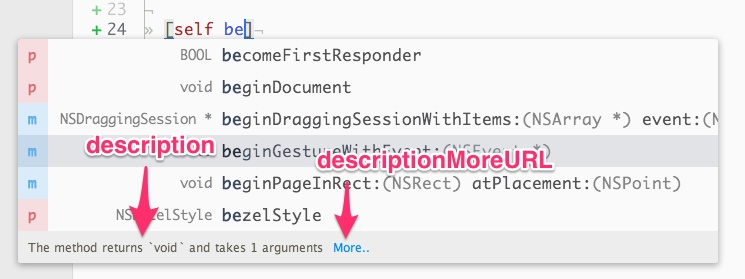
\includegraphics[width=\textwidth]{img/autocomplete.jpg}
\caption{\label{fig:autocomplete}Suggestions and possible customization.}
\end{figure}

Atom uses \texttt{autocomplete} package, which implements static and runtime autocompletion. The first one is based on grammar scopes. Every pattern that defines ''\texttt{support.*}'' scopes (\ref{list:scopes}) is used to generate a list of possible suggestions. Though patterns should be presented in form of enumeration. For example, the standard modules list is given: \texttt{(ssreflect|ssrfun|ssrbool|eqtype|ssrnat|div|prime|…)}.

Some languages may have context-sensitive things, like names of functions, variables, classes. To detect such entities, you need to write a parser, add type deduction (if required), and generate prompts. A~logical step is to connect the existing compiler, and refer to its internal representation, to the abstract syntax tree. The Coq compiler does not provide such information at the current moment (it is under discussion), but it will become possible in the future~\autocite{coq-autocompletion}.

When the user presses ctrl + space hotkey to get a list of prompts, the package calls the \texttt{getSuggestions} method. It takes four parameters: editor, bufferPosition, scopeDescriptor, prefix. The prefix is the prefix of the word that the user types, bufferPosition --- the position of the cursor in the text, scopeDescriptor is a scope described by patterns. The method returns a list of suggestions with additional customization (see~picture~\ref{fig:autocomplete}).

There is another type of helpers for users --- snippets. They are similar to autocompletion with the only difference being that the basic multiline language constructs are prompted, such as for loops, switch-case statements, function headers, empty classes with a constructor...

The Coq language is conditionally divided into two sublanguages. The first is {\em Vernacular}, a language for defining functions, algebraic types, modules, theorems. This language is relatively simple, there is a limited number of constructions described by a small grammar on less than 100 lines~\autocite{vernacular-grammar}. The second, {\em Gallina}, is used to describe the proofs of theorems. This language contains a huge number of tactics (functions), which number is about 226~\autocite{tactics-index}.

To support them all, it's best to write a documentation scrapper that will generate a grammar and snippets. So did the developers of the plugin for Emacs editor~\autocite{tactics-emacs}. They store tactics in the form \texttt{\{'("tactic~@\{hole1\}~@\{hole2\}"\}}, that can be easily converted into atom's representation:

\vspace{1em}
\begin{lstlisting}
    '.source.coq':
      'Definition ... := ...':
        "prefix": "Definition"
        "body":   "Definition $1 := $2."
\end{lstlisting}

\vspace{1em}
Prefix is used in a fuzzy search, when a user types in a word. Body is a content of the snippet, where \$1 is a hole, the user will be asked to fill. This snippet will be prompted at the ''\texttt{source.coq}'' scope.

In order not to offer 200 tactics in the place where they can not be used, two different scopes for gallina and vernacular were made, so that one is embedded into the other (see snippet~\ref{list:scopes}).

\section{Compiler dependent features}

To implement the rest of the features, some compiler interface is required. Fortunately, Coq developers provide this option with the help of two utilities. The newer one is {\em serapi}, actively developing at the moment, aimed at web-based applications. The authors tried to simplify the life of developers, hiding the internal structures of the compiler's implementation. Unfortunately, this utility is still damp, so it was decided to abandon it. Another way is an older interface, {\em coqtop}.

In fact, coqtop is an interactive environment for executing user commands, or in other words, REPL~--- run-eval-process loop. The flag ''\mbox{\texttt{main-channel stdfds -ideslave}}'' allows to  redirect the input and output streams so that they can be used from a third-party process. The following snippet shows how to run coqtop from a nodejs application.\\


\begin{ListingEnv}[H]
\begin{Verb}

var coqtop = require('child_process')
    .spawn(coqtop_path, ["-main-channel", "stdfds", "-ideslave"])
    
coqtop.on('exit', exitCode => ...)
coqtop.stderr.on('data', err => ...)
coqtop.stdout.on('data', data => ...)
\end{Verb}
\caption{How to run coqtop from nodejs}
\label{list:nodejs-run-coq}
\end{ListingEnv}

The event loop is what allows Node.js to perform non-blocking I/O operations. Therefore, when the child process responds, the callback from the last line will be called, without blocking the main process, that is, the code editor. To send data there is a command \texttt{coqtop.stdin.write()}.

\newpage


\subsection{Step by step compilation}

Coq is a language consisting of sentences, separated by dots. Each sentence is assigned a unique stateId after being sent to Coq (via \texttt{Add} method). State ID 0 is reserved as ''null'' or ''default'' state. If the sentence contains an error, then the new stateId will not be defined.

First, the coqtop must be initialized with the \texttt{Init} command. It sets the stateId to one. After the user has entered the next sentence, he can check its correctness. Obviously, at this point the editor should call the  \texttt{Add} method, get a new stateId and remember it.

At some point, the user may want to edit the previous sentence, for such cases there is an \texttt{editAt} method that takes stateId. First, the state can be saved if the user has deleted or added whitespace, since they do not affect anything. Second, to effectively obtain a stateId sentence on the position of the cursor in the text, two sorted lists can be used. The first to search by the line number, the second by the column number (if there are several sentences on one line).

Special behavior is observed in proofs. The fact is that as long as a theorem is not proved, every sentence-tactic will have its own stateId. But as soon as \texttt{Qed} is added, the entire proof becomes one term-sentence, and stateId is redefined.\\
\vspace{1em}
\begin{figure}[H]
\centering
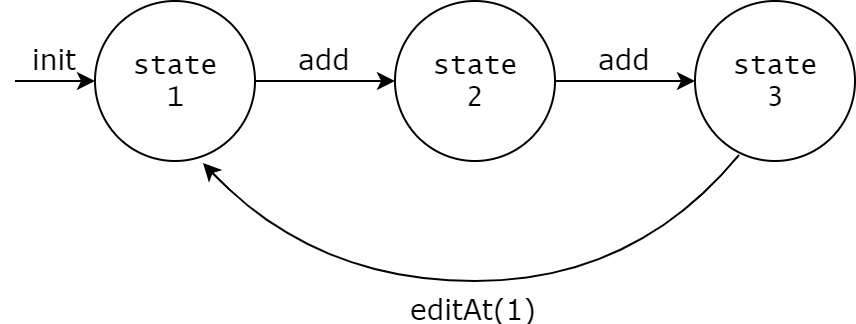
\includegraphics[width=28em]{img/dia.png}
\caption{\label{fig:dia}Coqtop is based on states connected with sentences.}
\end{figure}

\newpage

\subsection{Memorizing of computed results}

The main idea here is that when the user hovers a cursor over the sentence, the editor tries to calculate this sentence and returns the result. In case of proofs, goals should be displayed for the current sentence to help the user to trace the progress of the observable proof.

Coqtop contains two commands that could solve this problem. The first ''\texttt{Goal}'' returns a list of goals that need proof. For example:

\begin{lstlisting}
Goal P -> (1=1/\2=2) /\ 3=3.

intros. split;
(* goals are [1=1, 2=2, 3=3] *)

Focus 2.
(* current goal is [2=2]; bg-before: [1=1], bg-after: [3=3] *)
\end{lstlisting}

The other command is ''\texttt{Query}'', that performs queries on the currently focused state, and in fact simply processes the sentences. For example ''\texttt{Eval compute in 2+2.}'' will be evaluated as \mbox{''4 : nat''}.

The calculated results should be associated with sentences and have a quick access. For this, the data structure used in the previous subsection can be expanded to store the result along with the text of the sentence.

\subsection{Match cases generation based on type definitions}

Coq and many other functional languages have the notion of pattern-matching, the act of checking a given sequence of tokens for the presence of the constituents of some pattern. There is a special operator for this: \texttt{match \$expr} with ... end}. Where \texttt{\$expr} is an expression.

In some cases it is possible to generate the body for match operator by looking at the type of expression. Coqtop ''\texttt{MkCases}'' command returns a list of constructor names. For \texttt{nat} they are \texttt{O} and \texttt{S x}. Complex expressions can be preliminarily evaluated by \texttt{Query} command.

\newpage

\section{Plugin development}

In other text editors a user can compile a sentence by pressing shortcuts on the keyboard. Similar behavior can be implemented in Atom. In the file \texttt{keymap.cson} specifies a list of shortcuts and functions that should be called. These functions a written in a separate file using javascript language. The file defines an object with several fields: \texttt{activate}, \texttt{deactivate}, \texttt{serialize}, \texttt{deserialize}. The first two are called when Atom wants to load (unload) the package, the last two are used to save data into the internal storage.

All text operations are performed through the \texttt{TextBuffer} object. When compiling, you need to find the first dot from the previous compiled sentence. The \texttt{getText} method is used for this. In turn, the compilation should end with highlighting the text in green in case of success and red in case of failure. To do this, the marker is placed above the text.

\begin{lstlisting}
    marker = editor.markBufferRange(range)
    decoration = editor.decorateMarker(marker, 
        { type: 'highlight', class: 'success' })
\end{lstlisting}

Each marker has an invalidation tactic, which determines when it should be turned off: after changing the text inside, on the edges, in the line, etc. For our case, the tactic "inside" is suitable.



% And fully described at the Atom documentation~\autocite{atom-docs}


\newpage

\Conc

The approach to creating Atom language packages was investigated, and as a result the coq language plugin was developed. It supports minimal functionality for comfortable work and can potentially be improved. The source code is available at https://github.com/xamgore/language-coq.



% Печать списка литературы (библиографии)
\printbibliography[%{}
    heading=bibintoc%
    ,title=Bibliography % если хочется это слово
]
% Файл со списком литературы: biblio.bib
% Подробно по оформлению библиографии:
% см. документацию к пакету biblatex-gost
% http://ctan.mirrorcatalogs.com/macros/latex/exptl/biblatex-contrib/biblatex-gost/doc/biblatex-gost.pdf
% и огромное количество примеров там же:
% http://mirror.macomnet.net/pub/CTAN/macros/latex/contrib/biblatex-contrib/biblatex-gost/doc/biblatex-gost-examples.pdf

\appendix
\ifthenelse{\value{worktype} > 1}{%
  \addtocontents{toc}{%
      \protect\renewcommand{\protect\cftchappresnum}{\appendixname\space}%
      \protect\addtolength{\protect\cftchapnumwidth}{\widthof{\appendixname\space{}} - \widthof{Глава }}%
  }%
}{
  \addtocontents{toc}{%
      \protect\renewcommand{\protect\cftsecpresnum}{\appendixname\space}%
      \protect\addtolength{\protect\cftsecnumwidth}{\widthof{\appendixname\space{}}}%
  }%
}

\newpage
% \section{Пример работы программы}

% Здесь длинный листинг с примером работы.



















































% Если typeOfWork в SETUP.tex задан как 2 или 3, то начинать
% надо не с section (раздел), а с главы (chapter)
% \section*{Несколько примеров в~\LaTeX{}}
% \label{sec:examples}

% Некоторые часто используемые
% команды приведены в качестве примера ниже (и варианты — в
% комментариях). Мы рекомендуем внимательно прочесть данный
% текст и изучить его исходный код прежде, чем начинать писать
% свой собственный. Кроме того, можно дать и такой совет: идущий
% ниже текст не убирать до самого конца, а просто оставлять его
% позади своего собственного текста, чтобы в любой момент можно
% было проконсультироваться с данными примерами.

% \subsection*{Как вставлять листинги и рисунки}

% Для крупных листингов есть два способа. Первый красивый, но в нём не допускается
% кириллица (у вас может встречаться в комментариях и
% печатаемых сообщениях), он представлен на листинге~\ref{list:hwbeauty}.
% \begin{ListingEnv}[H]% буква H означает Here, ставим здесь,
% % элементы, которые нежелательно разрывать обычно не ставят
% % посреди страницы: вместо H используется t (top, сверху страницы),
% % или b (bottom) или p (page, на отдельной странице)
% \begin{lstlisting}
% #include <iostream>
% using namespace std;

% int main()
% {
%     cout << "Hello, world" << endl;
%     system("pause");
%     return 0;
% }
% \end{lstlisting}
% %следующую команду для генерации подписи можно опустить,
% % хотя рекомендуется все специальные элементы (таблицы, рисунки,
% % листинги) подписывать. Если подпись пропустить, листинг также не получит
% % номера и на него не сошлёшься в будущем
% \caption{Программа “Hello, world” на \protect\cpp}
% % далее метка для ссылки:
% \label{list:hwbeauty}
% \end{ListingEnv}

% Второй не такой красивый, но без ограничений (см.~листинг~\ref{list:hwplain}).
% \begin{ListingEnv}[H]
% \begin{Verb}

% #include <iostream>
% using namespace std;

% int main()
% {
%     cout << "Привет, мир" << endl;
% }
% \end{Verb}
% \caption{Программа “Hello, world” без подсветки}
% \label{list:hwplain}
% \end{ListingEnv}

% Можно использовать первый для вставки небольших фрагментов
% внутри текста, а второй для вставки полного
% кода в приложении, если таковое имеется.

% Если нужно вставить совсем короткий пример кода (одна или две строки), то выделение  линейками и нумерация может смотреться чересчур громоздко. В таких случаях можно использовать окружения \texttt{lstlisting} или \texttt{Verb} без \texttt{ListingEnv}. Приведём такой пример с указанием языка программирования, отличного от заданного по умолчанию:
% \begin{lstlisting}[language=Haskell]
% fibs = 0 : 1 : zipWith (+) fibs (tail fibs)
% \end{lstlisting}
% Такое решение~--- со вставкой нумерованных листингов покрупнее
% и вставок без выделения для маленьких фрагментов~--- выбрано,
% например, в книге Эндрю Таненбаума и Тодда Остина по архитектуре
% компьютера~ autocite{TanAus2013} (см.~рис.~\ref{fig:tan-aus}).

% Наконец, для оформления идентификаторов внутри строк
% (функция \lstinline{main} и тому подобное) используется
% \texttt{lstinline} или, самое простое, моноширинный текст
% (\texttt{\textbackslash texttt}).

% \begin{figure}[p]% p означает, что нужно выделить для рисунка
% % отдельную страницу; применяется для больших рисунков
% \centering
% %Здесь могла быть ваша лягушка.
% 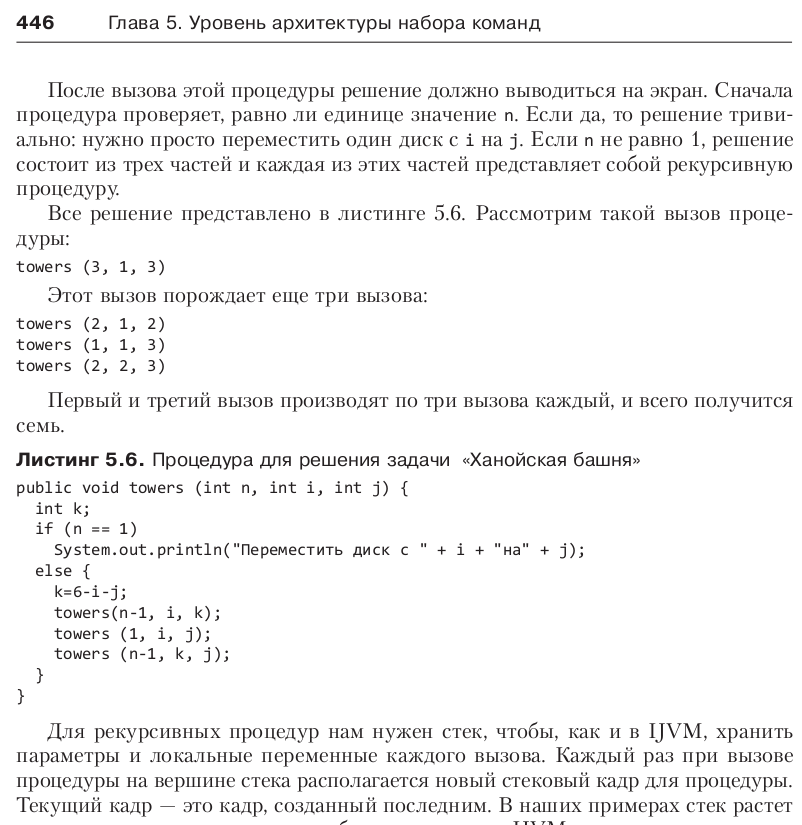
\includegraphics[width=\textwidth]{img/tan-aus.png}
% \caption{\label{fig:tan-aus}Пример оформления листингов в~ autocite{TanAus2013}}
% \end{figure}

% Использовать внешние файлы (например, рисунки) можно и на \href{http://overleaf.com}{overleaf.com}: ищите кнопочку upload.

% \subsection*{Как оформить таблицу}

% Для таблиц обычно используются окружения table и tabular --- см. таблицу~\ref{tab:widgets}. Внутри окружения tabular используются специальные команды пакета booktabs — они очень красивые; самое главное: использование вертикальных линеек считается моветоном.

% \begin{table}
% \centering
% \caption{\label{tab:widgets}Подпись к таблице --- сверху}
% \begin{tabular}{llr}
% \toprule
% \multicolumn{2}{c}{Item} \\
% \cmidrule(r){1-2}
% Животное  & Описание    & Цена (\$) \\
% \midrule
% Gnat      & per gram    & 13.65      \\
%           & each        & 0.01       \\
% Gnu       & stuffed     & 92.50      \\
% Emu       & stuffed     & 33.33      \\
% Armadillo & frozen      & 8.99       \\
% \bottomrule
% \end{tabular}
% \end{table}

% \subsection*{Как набирать формулы}

% \LaTeX{} is great at typesetting mathematics. Let $X_1, X_2, \ldots, X_n$ be a sequence of independent and identically distributed random variables with $\text{E}[X_i] = \mu$ and $\text{Var}[X_i] = \sigma^2 < \infty$, and let
% $$S_n = \frac{X_1 + X_2 + \cdots + X_n}{n}
%       = \frac{1}{n}\sum_{i}^{n} X_i$$
% denote their mean. Then as $n$ approaches infinity, the random variables $\sqrt{n}(S_n - \mu)$ converge in distribution to a normal $\mathcal{N}(0, \sigma^2)$.

% \subsection*{Как оформлять списки}

% Нумерованные списки (окружение enumerate, команды item)…

% \begin{enumerate}
%   \item Like this,
%   \item and like this.
% \end{enumerate}

% \dots маркированные списки \dots

% \begin{itemize}
%   \item Like this,
%   \item and like this.
% \end{itemize}

% \dots списки-описания \dots

% \begin{description}
%   \item[Word] Definition
%   \item[Concept] Explanation
%   \item[Idea] Text
% \end{description}

% \section*{Заключение}

% Помните, что на все пункты списка литературы должны быть ссылки. \LaTeX\ просто не добавит информацию об издании из bib"/файла, если на это издание нет ссылки в тексте. Часто студенты используют в работе  электронные ресурсы: в этом нет ничего зазорного при одном условии: при каждом заимствовании следует ставить соответствующую ссылку. В качестве примера приведём ссылку на сайт нашего института~ autocite{mmcs}.

% Для дальнейшего изучения \LaTeX\ рекомендуем книгу Львовского~ autocite{Lvo2003}: она хорошо написана, хотя и несколько устарела.
% Обычно стоит искать подсказки на
% \href{http://tex.stackexchange.com/}{tex.stackexchange.com}, а также
% читать документацию по установленным пакетам с помощью
% команды
% \begin{Verb}
% texdoc имя_пакета
% \end{Verb}
% или на \href{http://ctan.org/}{ctan.org}. s





\end{document}
